\chapter{Theory}
\section{Background Theory}
\subsection{Theory about the Sun}
Statification

\subsection{Mixing length theory}
\subsection{Perturbation theory}

\section{Anelastic MHD}
\subsection{General anelastic MHD}




\subsection{Ideal anelastic MHD}



\subsection{Timestepping}

\section{Numerical Methods}
\subsection{Discretization}
\subsection{Simulation Box}
\subsection{Temporal Methods}
\subsection{Spatial Methods}




\subsection{Stability Analysis}

We will use Von Neumann analysis of the advection equation to determine the required time-step sizes for our solver. The advection equation is
\begin{equation}
    \frac{\partial u(t,x)}{\partial t} = -a \frac{\partial u(t,x)}{\partial x},
\end{equation}
where $u(t,x)$ is the exact solution and $a$ is constant representing the velocity. This is discretized over a grid such that $y(t_n,x_j)=y_{n,j}$, where $t_n = n\Delta t$ and $x_j = j\Delta x$ for $n,j\in\mathbb{N}$, is our numerical solution. The advection equation then becomes

\begin{equation}
    \left[\frac{\partial y}{\partial t}\right]_{n,j} = -a \left[\frac{\partial y}{\partial x}\right]_{n,j}.
\end{equation}
The numerical solution is
\begin{equation}
    y_{n,j} = u(t_n,x_j)+\epsilon_{n,j},
\end{equation}
where $\epsilon_{n,j}$ is the round-off error. The round-off error must also satisfy the discretized equation and this gives us that
\begin{equation}\label{eq:advection_error}
    \left[\frac{\partial \epsilon}{\partial t}\right]_{n,j} = -a \left[\frac{\partial \epsilon}{\partial x}\right]_{n,j}.
\end{equation}
We expand the round-off error as a fourier series
\begin{equation}
    \epsilon(t_n,x_j) = \sum_m E_m(t_n) e^{i k_m j\Delta x},
\end{equation}
where $k_m$ is the wavenumber and $E_m(t_n)$ is the time-dependent amplitude of the error. When inserting this into our differential equation we get a linear difference equation, meaning that each of the terms behave like the entire series, so we can consider the growth of only one term
\begin{equation}
    \epsilon_m(t_n,x_j) = E_m(t_n) e^{i k_m j\Delta x}.
\end{equation}
We will show the calculations using the first-order upwind scheme with the second-order Runge-Kutta scheme. Since this should be true for any $m$ we remove the subscipt, define $\beta\equiv k\Delta x$ and get that the spacial derivative is
\begin{align*}
    \left[\frac{\partial \epsilon}{\partial x}\right]_{n,j} &= \frac{\epsilon_{n,j}-\epsilon_{n,j-1}}{\Delta x}\\
    &= \frac{E(t_n) e^{i \beta j}- E(t_n) e^{i \beta (j-1)}}{\Delta x}\\
    &= E(t_n)e^{i\beta j} \frac{1-e^{-i\beta}}{\Delta x}.
\end{align*}
This gives us that the advection equation \ref{eq:advection_error} becomes
\begin{align}
    \left[\frac{\partial \epsilon}{\partial t}\right]_{n,j} = e^{i\beta j}\left[\frac{\partial E(t_n)}{\partial t}\right]_{n,j} &= -a E(t_n)e^{i\beta j} \frac{1-e^{-i\beta}}{\Delta x}\\
    \left[\frac{\partial E(t_n)}{\partial t}\right]_{n,j} &= -a E(t_n)\frac{1-e^{-i\beta}}{\Delta x}.
\end{align}
We define $\lambda= - \frac{a}{\Delta x}\left( 1-e^{-i\beta} \right)$ which gives us 
\begin{equation}
    \mu = \Delta t \lambda = - C\left( 1-e^{-i\beta} \right),
\end{equation}
where $C\equiv a\Delta t/\Delta x$ is the Courant number. This means that the differential equation for the time-dependent error is
\begin{equation}
    \left[\frac{\partial E(t_n)}{\partial t}\right]_{n,j} = \lambda E_n.
\end{equation}
Using this with the second order Runge-Kutta scheme, the slopes for the time-dependent error is
\begin{align*}
    k_1 &= \lambda E_n,\\
    k_2 &= \lambda \left(E_n+\frac{\Delta t}{2}k_1 \right) = E_n \left( \lambda + \Delta t \lambda^2 \right).
\end{align*}
And the next time-step for the error is
\begin{align*}
    E_{n+1} &= E_n + \Delta t \left( \frac{k_1}{2} +\frac{k_2}{2} \right)\\
    &= E_n \left( 1 +\Delta t \lambda + \frac{1}{2}\left( \Delta t\lambda \right)^2 \right)\\
    & = E_n \left( 1 + \mu + \frac{1}{2}\mu^2  \right).
\end{align*}
This gives us the amplification factor 
\begin{equation}
    g = \frac{E_{n+1}}{E_n} = \left( 1 + \mu + \frac{1}{2}\mu^2  \right).
\end{equation}
We require $|g|\leq 1$, meaning that the time-dependent error does not grow in time. If this is any bigger than $1$ the error will grow exponentially, giving an unstable numerical solution. Following the same steps for some other schemes we get the following equations for spacial schemes:
\begin{align*}
    \text{First order upwind} &: \mu=-C\left(1-e^{-i\beta}\right),\\
    \text{Second order upwind} &: \mu=-\frac{C}{2}\left(3-4e^{-i\beta}+e^{-2i\beta}\right),\\
    \text{Second order central} &: \mu = -\frac{C}{2}\left(e^{i\beta} - e^{-i\beta}\right),\\
    \text{Fourth order central} &: \mu = - \frac{C}{12}\left(-e^{2i\beta}+8e^{i\beta}-8e^{-i\beta}+e^{-2i\beta}\right).
\end{align*}
And for the temporal schemes:
\begin{align*}
    \text{First order RK} &: g = 1+\mu,\\
    \text{Second order RK} &: g = 1+\mu + \frac{1}{2}\mu^2,\\
    \text{Third order RK} &: g = 1+\mu + \frac{1}{2}\mu^2+\frac{1}{6}\mu^3,\\
    \text{Fourth order RK} &: g = 1+\mu + \frac{1}{2}\mu^2+\frac{1}{6}\mu^3+\frac{1}{24}\mu^4.
\end{align*}
In figures \ref{fig:vn_rk1}, \ref{fig:vn_rk2}, \ref{fig:vn_rk3} and \ref{fig:vn_rk4} we see the amplification factor for different $C$ and $\beta$. Using the periodicity of $\beta$ we can pick $\Delta x$ and a corresponding $\Delta t$ given the magnitude of $a$.
\begin{figure}[htbp]
    \centering
    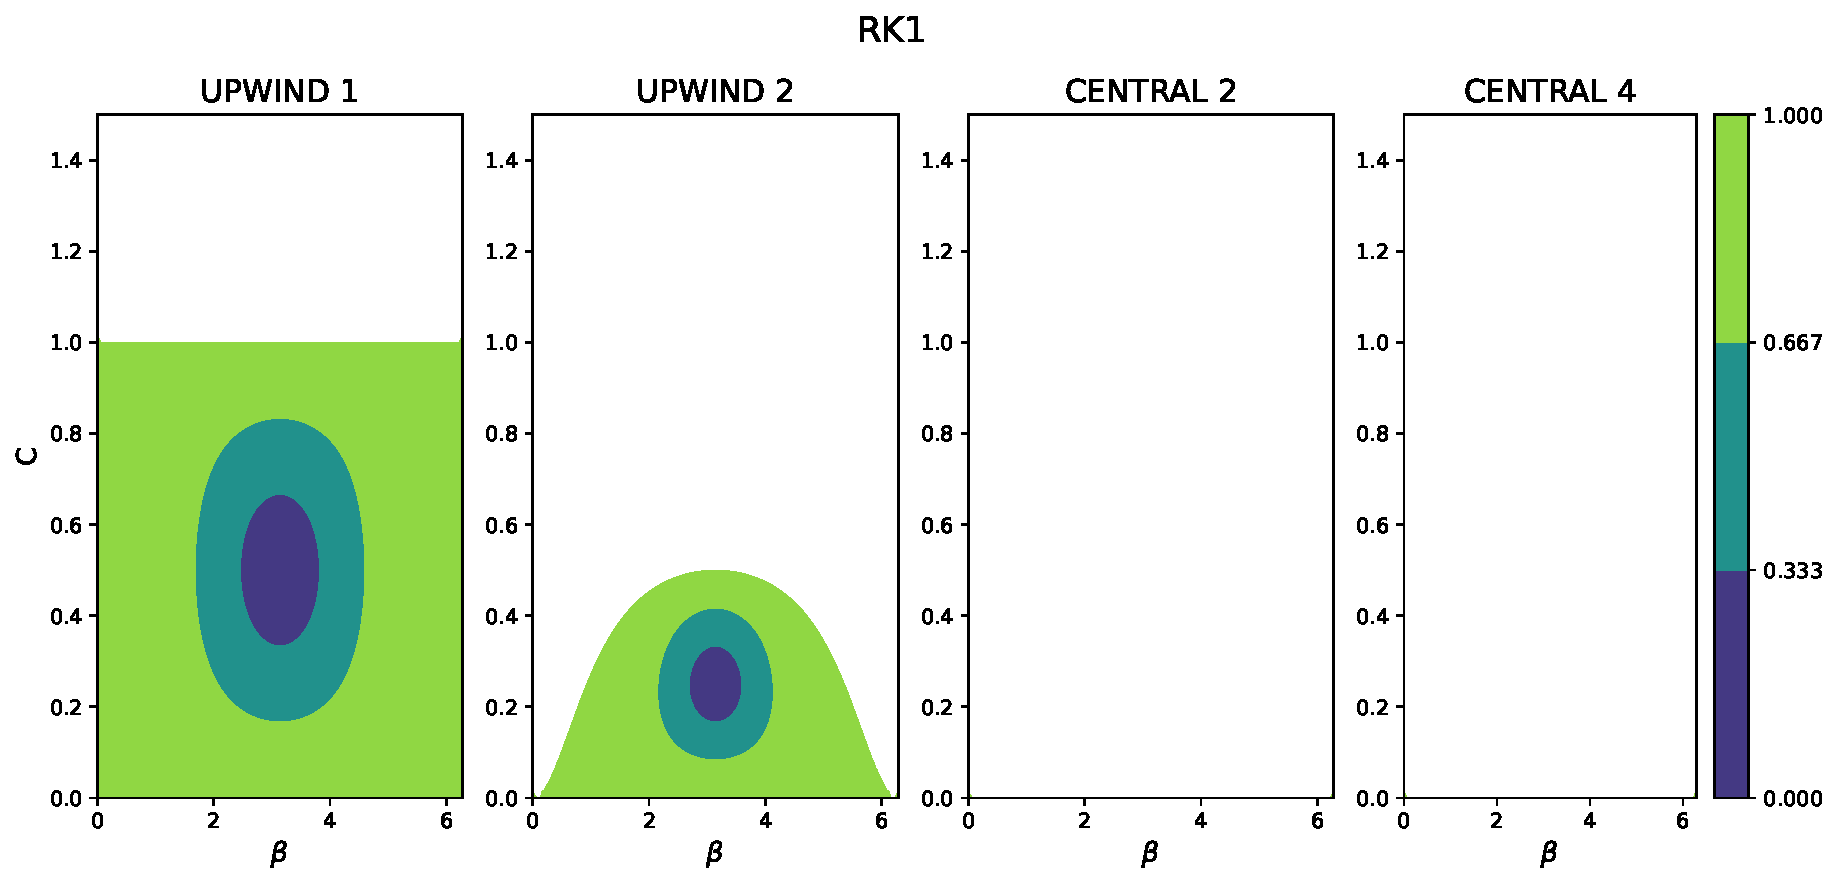
\includegraphics[width=0.8\linewidth]{./von_neumann_figs/vn_rk1.pdf} % Adjust the width as necessary
    \caption{Amplification factor magnitude for the first-order Runge Kutta scheme.}
    \label{fig:vn_rk1} % For referencing the figure elsewhere in your document
\end{figure}
\begin{figure}[htbp]
    \centering
    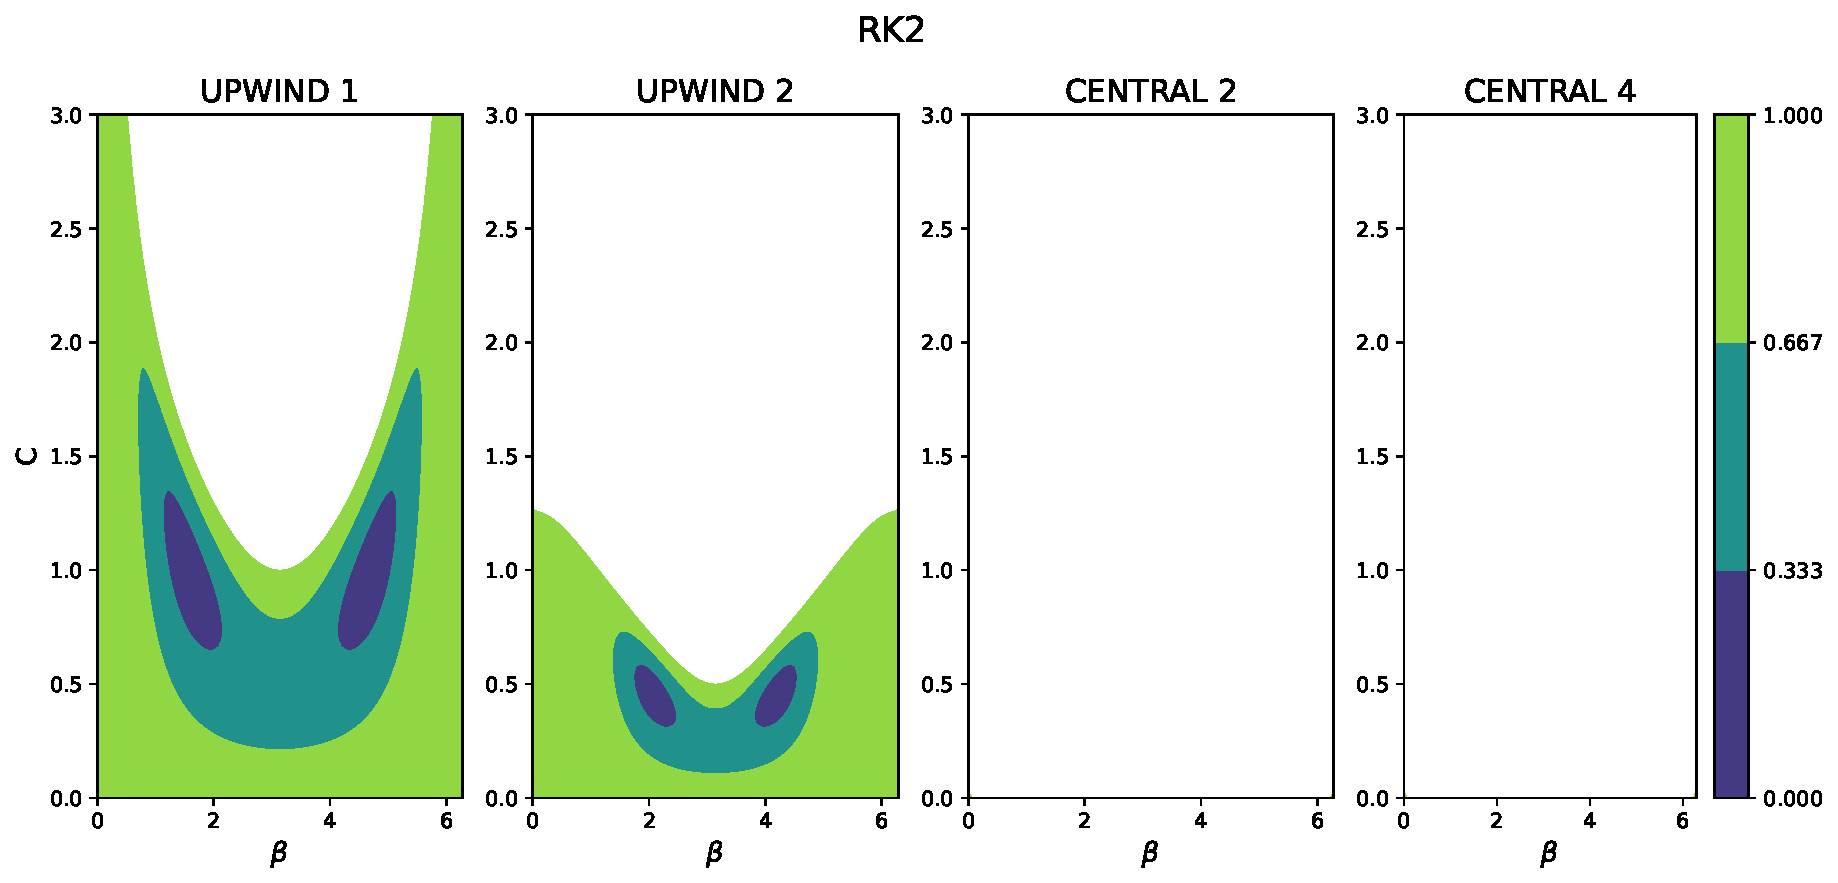
\includegraphics[width=0.8\linewidth]{./von_neumann_figs/vn_rk2.pdf} % Adjust the width as necessary
    \caption{Amplification factor magnitude for the second-order Runge Kutta scheme.}
    \label{fig:vn_rk2} % For referencing the figure elsewhere in your document
\end{figure}
\begin{figure}[htbp]
    \centering
    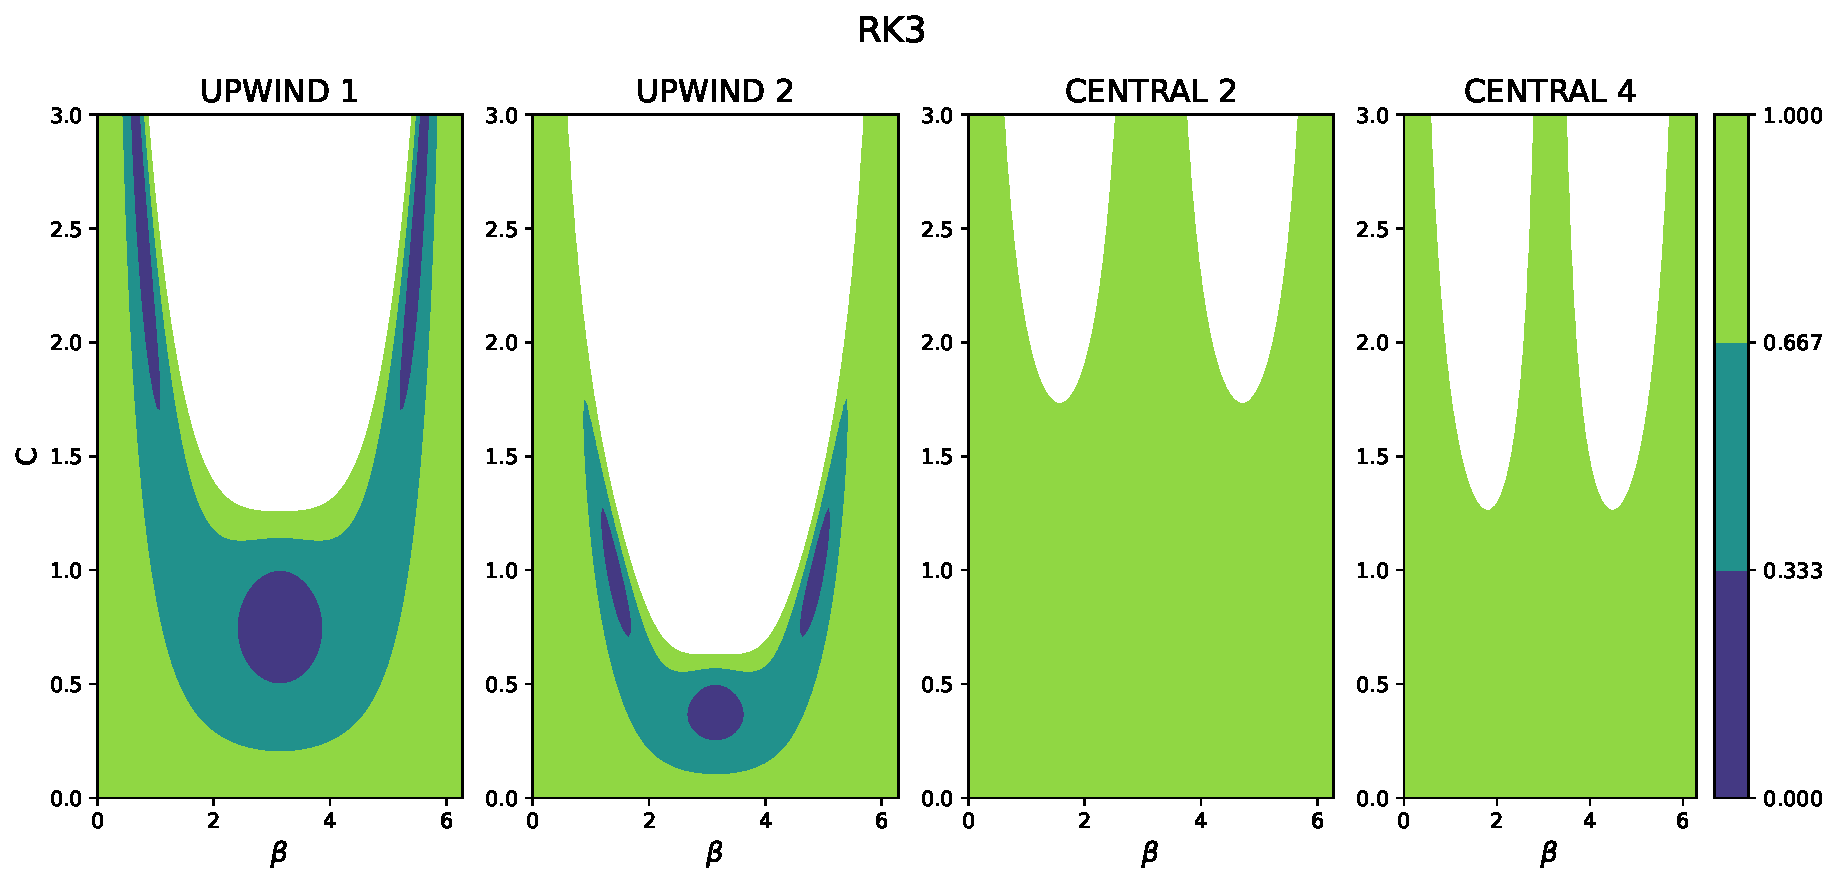
\includegraphics[width=0.8\linewidth]{./von_neumann_figs/vn_rk3.pdf} % Adjust the width as necessary
    \caption{Amplification factor magnitude for the third-order Runge Kutta scheme.}
    \label{fig:vn_rk3} % For referencing the figure elsewhere in your document
\end{figure}
\begin{figure}[htbp]
    \centering
    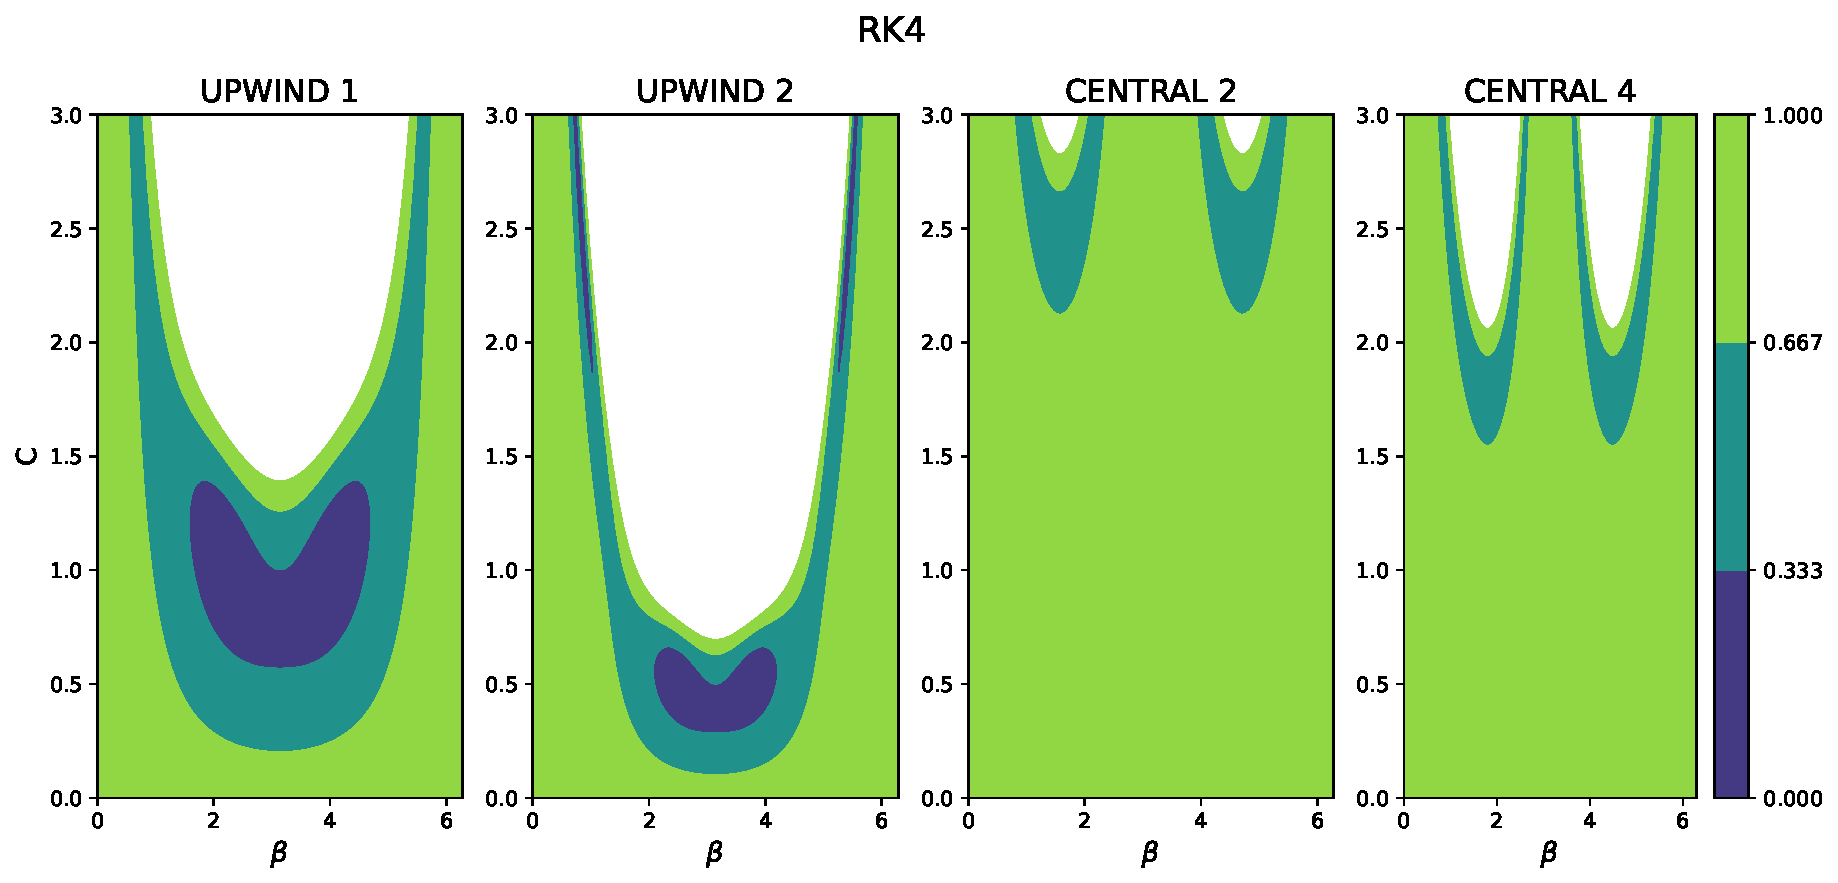
\includegraphics[width=0.8\linewidth]{./von_neumann_figs/vn_rk4.pdf} % Adjust the width as necessary
    \caption{Amplification factor magnitude for the fourth-order Runge Kutta scheme.}
    \label{fig:vn_rk4} % For referencing the figure elsewhere in your document
\end{figure}









\subsection{Background Initialization}

We base our background on reference values from the standard solar model, Solar S, \citep{1996Sci...272.1286C}. This data is downloaded from \href{https://users-phys.au.dk/~jcd/solar_models/cptrho.l5bi.d.15c}{https://users-phys.au.dk/~jcd/solar_models/cptrho.l5bi.d.15c} at 31.08.2023. The reference values for density $\rho_0(r_r)$, temperature $T_0(r_r)$ and pressure $p_0(r_r)$ are picked at a radius $r_r=0.71R_{\odot}$, which is the bottom of the convection zone \citep{1991ApJ...378..413C}. The mass at this point is calculated by
    \begin{equation}
        m(r_r)=\int_0^{r_r} dm = 4\pi \int_0^{r_r} \rho(r')r'^2 dr',
    \end{equation}
using cumulative trapezoidal integration. Having this we can use the following equations to integrate up and down from the reference point.

We are using an ideal gas model and therefore can not use this data as our entire background. This is because the temperature gradient of the background would not be large enough to produce convection numerically. Instead we will integrate out from our reference values and create a hydrostatic background. We will force convective instability by setting the superadiabaticity parameter 
    \begin{equation*}
        \Delta\nabla = \left(\frac{\partial\ln T}{\partial\ln p} \right)_{*} - \left(\frac{\partial\ln T}{\partial\ln p} \right)_{ad} = \nabla_{*} -\nabla_{ad} > 0,
    \end{equation*}
where $\nabla_{*}$ is the adiabatic temperature gradient of the star and $\nabla_{ad}=0.4$ is the adiabatic temperature gradient for an ideal gas. We therefore set 
    \begin{equation*}
    \nabla_{*} -\nabla_{ad} = 
        \begin{cases} 
        k & \text{if } r \geq 0.7 R_{\odot} \\
        0 & \text{if } r < 0.7 R_{\odot}
        \end{cases}
    \end{equation*}
For an ideal gas we have $\nabla_{ad}=0.4$ and we can then integrate our variables using the following equations.

\textbf{Mass of shell with thickness $dr$}
\begin{equation}\label{eq:mass_shell}
    \frac{dm}{dr} = 4\pi r^2\rho_0(r).
\end{equation}

\textbf{Hydrostatic equilibrium condition}
    \begin{equation}\label{eq:hydrostatic_equilibrium}
        \frac{ p_0}{ r} = -\frac{G m(r)}{r^2}\rho_0(r),
    \end{equation}
where $G$ is Newtons gravitational constant.

\textbf{????}
    \begin{equation}\label{eq:dT_dr}
        \frac{d T_0}{d r} = \nabla_{*} \frac{T_0}{p_0}\frac{d p_0}{d r}. 
    \end{equation}

We also have the \textbf{entropy gradient}
    \begin{equation*}
        \frac{ds}{dr} = -\frac{c_p}{H} \Delta\nabla,
    \end{equation*}
where the pressure scale height
    \begin{equation*}
        H = - \frac{dr}{d\ln p_0} = - p_0\frac{dr}{dp_0},
    \end{equation*}
the spesific heat capacity at constant pressure \citep{1999ApJS..121..247L}
    \begin{equation*}
        c_p = \frac{r_*}{1-1/\gamma},
    \end{equation*}
and $r_*$ is the spesific gas constant and $\gamma$ is the adiabatic parameter. The gas constant is taken from the ideal gas law on the from
    \begin{equation*}
        p = \frac{k_B}{\mu m_u} T,
    \end{equation*}
where $k_B$ is Boltzmanns constant $m_u$ is the atomic mass unit and $\mu$ is the mean molecular mass. Using the chemical abundaces of Hydrogen $\text{Ab(H)}=12$, Helium $\text{Ab(He)}=10.93$ and metals $\text{Ab(Metals)}=0.012$ \citep{2007SSRv..130..105G} we can calculate their number densities by 
    \begin{equation*}
        n_E = 10^{\text{Ab(E)}},
    \end{equation*}
the mass densities
    \begin{equation*}
        \rho_E = n_E\cdot m_E,
    \end{equation*}
where $m_e$ is the mass of the element, and the fractional abundance
    \begin{equation*}
        X_E = \frac{\rho_E}{\rho} = \frac{n_E m_E}{\sum_i n_i m_i},
    \end{equation*}
where $\rho$ is the total density. This gives us that $n_\text{H}=10^{12}$, $n_\text{He}=10^{10.93}$ and $n_\text{metals} = 10^{0.012}\approx1$. For simplification we firstly approximate $n_\text{metals}=0$, since $n_\text{metals}\approx1 \ll n_\text{H},n_\text{He}$, secondly $m_\text{He}\approx 4m_\text{H}$ and thirdly $m_\text{H}\approx m_u$. Then the the fractional abundance for Hydrogen, Helium and metals are
    \begin{align*}
        X_\text{H} &= \frac{n_\text{H}}{n_\text{H}+4 n_\text{He}} \approx 0.746,\\
        X_\text{He} &= \frac{n_\text{He}}{n_\text{H}+4n_\text{He}}\approx 0.063, \\
        X_\text{metals} &= 1 - X_{\text{H}} - X_\text{He} \approx 0.190
    \end{align*}
We will assume full ionization due to the high temperatures and densities of the convection zone as can be seen in figures \ref{fig:temperature} and \ref{fig:pressure} from the standard solar model. Then the total number of particles due to Hydrogen is 
\begin{equation*}
    \frac{2X_\text{H}\rho}{m_u},
\end{equation*}
by one proton and electron. The total number of particles due to Helium is
\begin{equation*}
    \frac{3 X_\text{He}\rho}{4 m_u},
\end{equation*}
by one alpha particle and two electrons. The metals will have one nucleus and a number of electrons equal to the number of protons in the nucleus per particle. This means that the ratio of free particles to the number of particles in the nucleus is always $(Z+1)/A$, where $Z$ is the number of protons and $A$ is the atomic weight. We can approximate this to $Z/A\approx 1/2m_u$ and get that the total number of particles due to the metals is
\begin{equation*}
    \frac{X_\text{metals}\rho}{2m_u}.
\end{equation*}
Then the total number of particles
\begin{equation*}
    n_{total} = \frac{\rho}{m_u}\left( 2X_\text{H} + \frac{3 X_\text{He}}{4} + \frac{X_\text{metals}}{2} \right).
\end{equation*}

This gives us the mean molecular weight per particle
\begin{equation}
    \mu = \frac{1}{2X_\text{H} + 3X_\text{He}/4 + X_\text{metals}/2}\approx 0.61.
\end{equation}

We can then calculate the spesific gas constant 
    \begin{equation*}
        r_* = \frac{k_B}{m_u \mu},
    \end{equation*}
and the \textbf{entropy gradient}
    \begin{equation}\label{eq:entropy_gradient}
        \frac{ds}{dr} = p_0 \frac{k_B}{\mu m_u}\frac{\Delta\nabla}{1-1/\gamma}\frac{dp_0}{dr}.
    \end{equation}
We integrate this up to a radius $r_e$ and down to a radius $r_b$, limiting $dr$ for numerical stability. The limitation on $dr$ is implemented by picking a $p<1$ such that 
    \begin{equation*}
        dr = \frac{pV}{f},
    \end{equation*}
for a variable $V$ with
    \begin{equation*}
        f = \frac{dV}{dr}.
    \end{equation*}
This is done for all the variables and the smalles $dr$ is picked. For updating the density in each grid point we use the ideal gas \textbf{equation of state}
    \begin{equation}\label{eq:eos}
        \rho = \frac{p}{T}\frac{m_u \mu}{k_B}.
    \end{equation}

When we have the background set up we can interpolate this to a grid. We have done this using linear interpolation and the comparrison between our background model and the Solar S model from radius $r=0.6R_{\odot}$ to $0.97R_{\odot}$ can be seen in figures \ref{fig:temperature} for temperature, \ref{fig:pressure} for pressure, \ref{fig:density} for density and \ref{fig:gravitationa_acceleration} for gravitational acceleration.

\begin{figure}[htbp]
    \centering
    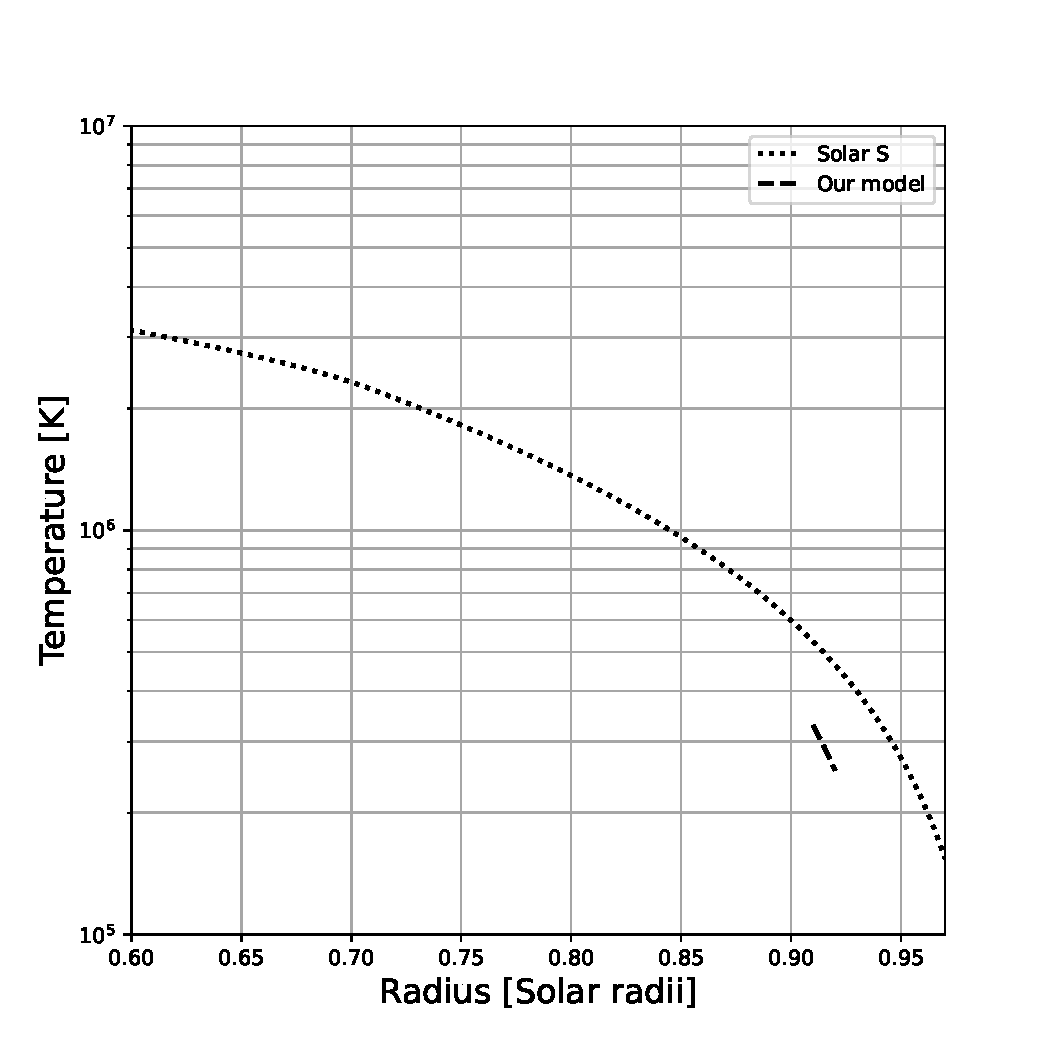
\includegraphics[width=0.8\linewidth]{./solar_vs_model_plots/Temperature.pdf} % Adjust the width as necessary
    \caption{Temperature as a function of radius for the integrated hydrostatic model in dashed lines and the Solar S model in dotted line.}
    \label{fig:temperature} % For referencing the figure elsewhere in your document
\end{figure}

\begin{figure}[htbp]
    \centering
    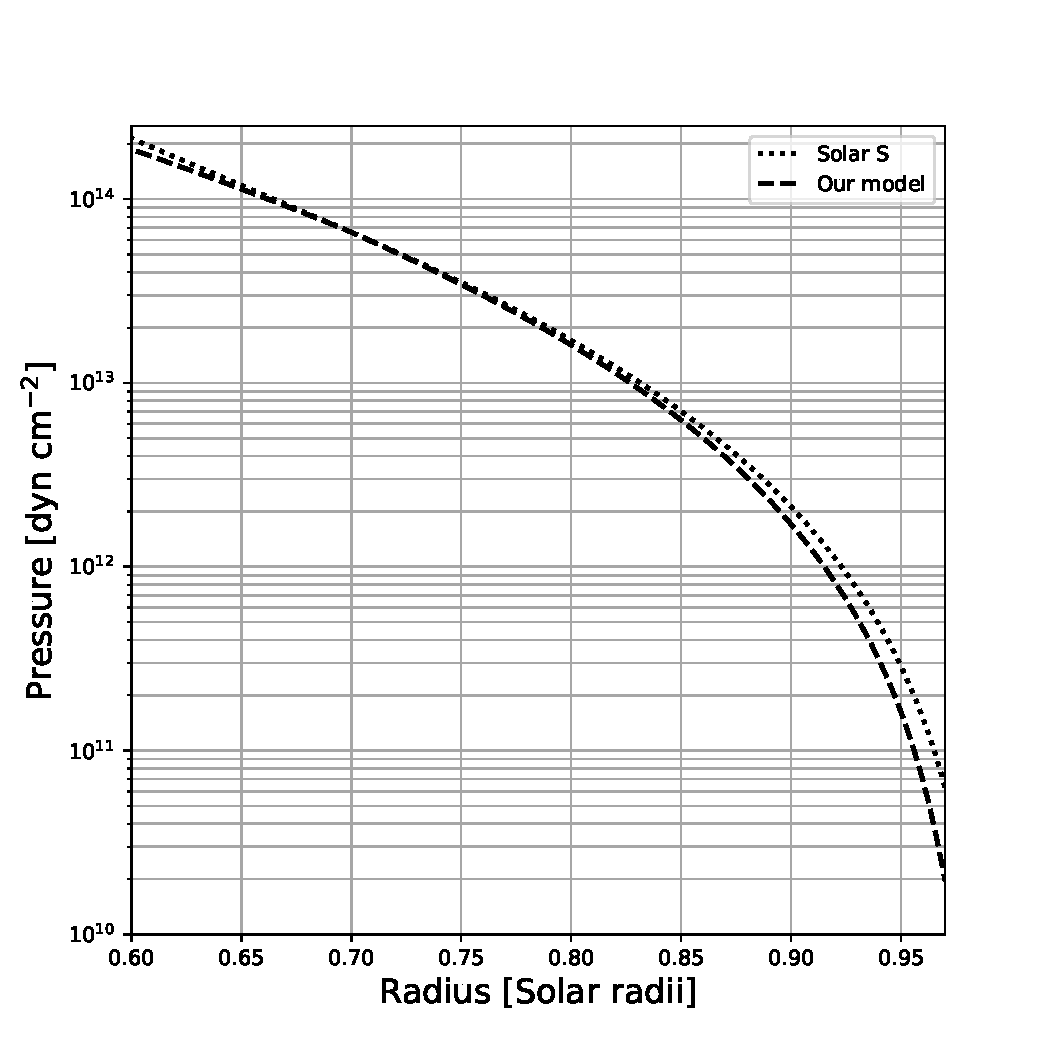
\includegraphics[width=0.8\linewidth]{./solar_vs_model_plots/Pressure.pdf} % Adjust the width as necessary
    \caption{Pressure as a function of radius for the integrated hydrostatic model in dashed lines and the Solar S model in dotted line.}
    \label{fig:pressure} % For referencing the figure elsewhere in your document
\end{figure}

\begin{figure}[htbp]
    \centering
    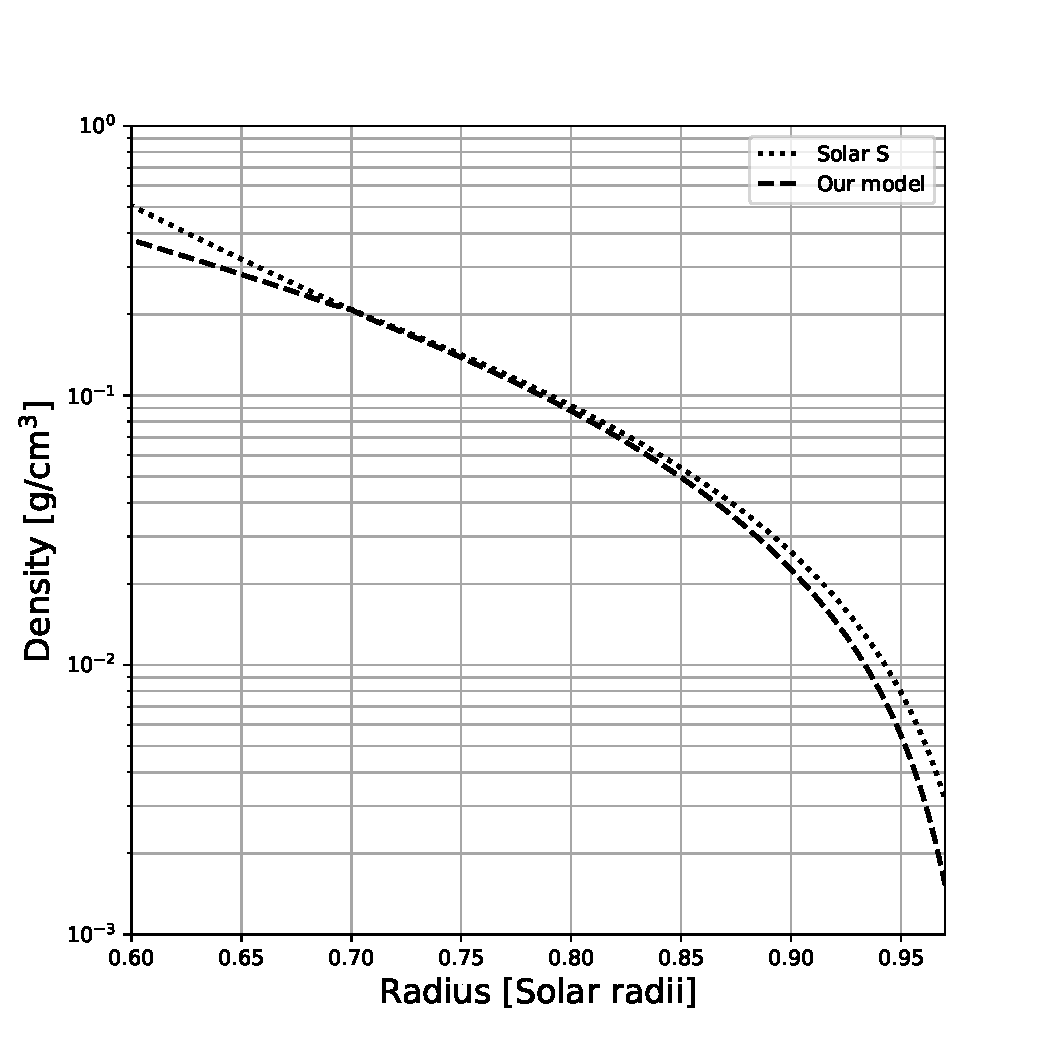
\includegraphics[width=0.8\linewidth]{./solar_vs_model_plots/Density.pdf} % Adjust the width as necessary
    \caption{Density as a function of radius for the integrated hydrostatic model in dashed lines and the Solar S model in dotted line.}
    \label{fig:density} % For referencing the figure elsewhere in your document
\end{figure}

\begin{figure}[htbp]
    \centering
    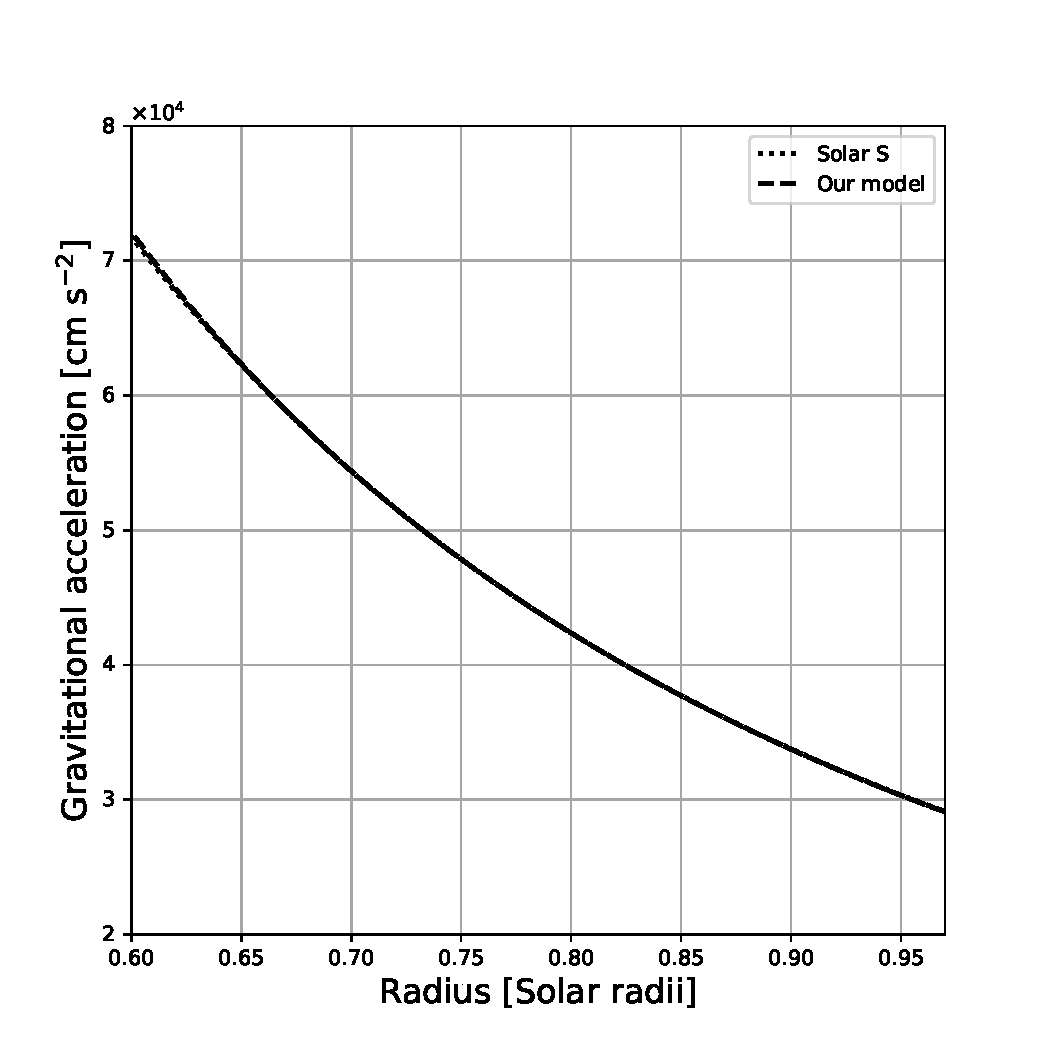
\includegraphics[width=0.8\linewidth]{./solar_vs_model_plots/Gravitational_acceleration.pdf} % Adjust the width as necessary
    \caption{Gravitational acceleration as a function of radius for the integrated hydrostatic model in dashed lines and the Solar S model in dotted line.}
    \label{fig:gravitationa_acceleration} % For referencing the figure elsewhere in your document
\end{figure}